\documentclass[]{scrartcl}
\usepackage[utf8]{inputenc}
\usepackage{graphicx}
\usepackage{amsmath}
\usepackage{float}
\usepackage[ngerman, english]{babel} 
\usepackage{hyperref}
\hypersetup{
	colorlinks,
	citecolor=black,
	filecolor=black,
	linkcolor=black,
	urlcolor=black,
}
\selectlanguage{ngerman}

\title{Modellierung dynamischer Systeme  \\ Abgabe der Praktikumsaufgabe 2}

\author{Maria Lüdemann und Birger Kamp}

\begin{document}

\maketitle
\selectlanguage{ngerman}
\tableofcontents
\newpage


\section{Teilaufgabe 1 - Erdumkreisung, Fluchtgeschwindigkeit und geostationäre Bahn}
In dieser Aufgabe ist es das Ziel den Flug eines Satelliten zu modellieren die von einer Trägerrakete in eine Startposition $x0$ gebracht wird. Von dort soll der Satellit antriebslos mit einer Geschwindigkeit von $v0$ und einem Flugwinkel $\Theta$ weiterfliegen und die Erde umrunden. Ab der antriebslosen Phase $x0$ startet unsere Simulation. Dabei haben wir wie vorgegeben den Einfluss des Satelliten auf die Erde vernachlässigt und die Simulation mithilfe des gegeben MatLab-Skripts $Erdbahn.m$ visualisiert. Die gegeben Werte werden in Abb \ref{fig:1_BezeichnerDiagramm} veranschaulicht. Für die Simulation wurde aus den gegeben Werten und angeforderten Funktionen ein Simulink Schaltbild entworfen das die Simulation durchführt.

\begin{figure}[H]
\centering
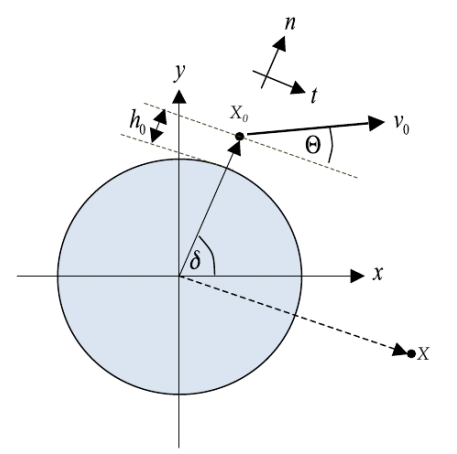
\includegraphics[width=0.5\linewidth]{./1_BezeichnerDiagramm}
\caption{}
\label{fig:1_BezeichnerDiagramm}
\end{figure}

\subsection{Gegebene Formeln und Konstanten}
Kraft auf den Satelliten
\begin{align}
\vec{F}_{S} = G \cdot \dfrac{m_{E} \cdot m_{S}}{r^2} \cdot \vec{e}_{SE}
\end{align}

Erdradius
\begin{align}
r_{E} = 6378 km
\end{align}

Erdmasse
\begin{align}
m_{E} = 5,9736 \cdot 10^{24} kg
\end{align}

Gravitationskonstante
\begin{align}
G = 66,743 \cdot 10^{-12} m^{3} kg^{-1} s^{-2}
\end{align}

\subsection{Konfigurierbare Parameter}
Folgende Parameter müssen mindestens bei der Simulation konfigurierbar sein:
\begin{itemize}
\item $v_{0}$ Startgeschwindigkeit $[km/s]$
\item $\Theta$ Flugwinkel $[^\circ]$
\item $\delta$ Startwinkel $[^\circ]$
\item $h_{0}$ Starthöhe $[km]$
\end{itemize}

\subsection{Funktionen}
Im Folgenden werden die benötigten Funktionen erklärt.

\subsubsection{Startposition}
Die Funktion Startposition berechnet den Startpositionsvektor $x0$ aus den gegeben Parametern $\gamma (^\circ)$ ,der Starthöhe $h0$ (km) und der Konstante Erdradius.

Dafür verwenden wir eine Formel die sich aus der Geometrie ableitet da hier mithilfe der Winkel die Ankathete und Gegenkathete der Hypotenuse von $r + h0$ berechnet werden aus denen sich die Position ableiten lässt.

Die Formel dazu beschreibt sich als 
\begin{align}
\vec{x} = [cos(\delta) \cdot( r + h0), sin(\delta) \cdot (r + h0)]
\end{align}

\subsubsection{vStart}
Die Funktion $vStart$ berechnet den Startgeschwindigkeitsvektor $\vec{v0}$ aus dem Startpositionsvektor $v0$, dem Flugwinkel $/Theta$ und dem durch die Funktion $Startposition$ berechneten Startpositionsvektor $x0$.

Um den Vektor bestimmen zu können werden zuerst die Einheitsvektoren in Tangential- und Normalrichtung ($\vec{t}, \vec{n}$ aus $x0$ konstruiert. Danach werden die Tangential- und Normalkomponenten der Startgeschwindigkeit ($v_t , v_n$) berechnet. Aus diesen Parametern lässt sich dann die Startgeschwindigkeit zusammenbauen.

Die genaue Durchführung findet sich im MatLab Code

\subsubsection{Beschleunigung}
Diese Funktion berechnet aus der Satellitenposition $\vec{x}$ die Satellitenbeschleunigung.
Die Kräfte die auf den Satelliten wirken summieren sich. 
\begin{align}
\Sigma{F} = m \cdot a
\end{align}
Daraus ergibt sich 

\begin{align}
a = \dfrac{\Sigma{F}}{m}
\end{align}

Wobei hier $m$ die Masse des Satelliten ist und sich heraus kürzt. Daraus folgt:

\begin{align}
a = \Sigma{F}_{SE}
\end{align}

Daraus ergibt sich

\begin{align}
a = G \cdot \dfrac{m_E \cdot m_S }{r^2_{SE}} \cdot \vec{e_{SE}}
\end{align}

hierbei ist $m_E$ die Masse der Erde, $m_S$ die Masse des Satelliten, $G$ die Gravitationskonstante, $\vec{e_{SE}}$  der Einheitsvektor vom Satelliten zur Erde und $r_{SE}$ der Abstand vom Erdmittelpunkt zum Satelliten. Auch hier ist die Masse des Satelliten vernachlässigbar und wird in der Berechnung nicht berücksichtigt.

\subsubsection{Kontakt}

Der Kontakt ist eine recht simple Funktion deren Aufgabe es ist festzustellen ob der Satellit einen Erdkontakt hergestellt hat. Dies wird verwendet um die Simulation zu beenden wenn der Satellit abgestürzt ist.

Die Funktion benutzt den aktuellen Positionsvektor des Satelliten $\vec{x}$ um daraus zu bestimmen ob die aktuelle Höhe größer ist als der Radius der Erde $r_E$.

\subsection{Simulink-Modell}

Das folgende Modell veranschaulicht das Simulink-Modell das die Simulation durchführt.

\begin{figure}[H]
\centering
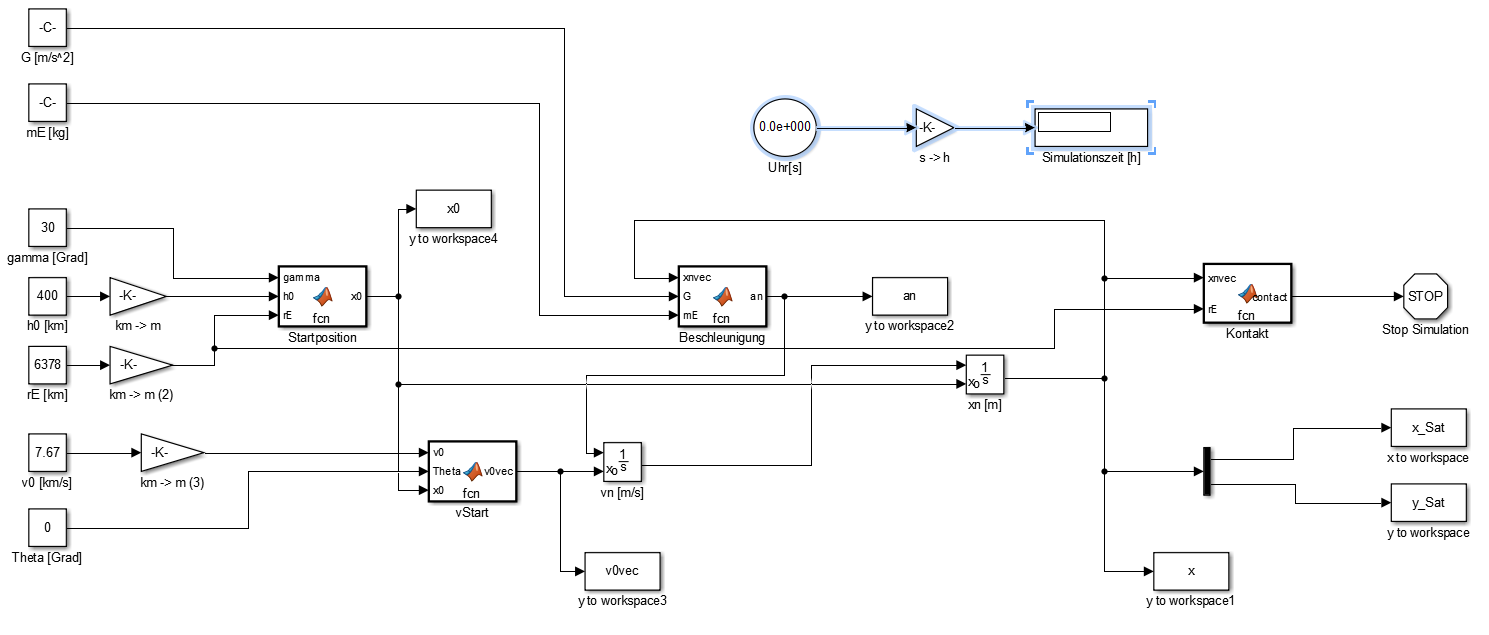
\includegraphics[width=1\linewidth]{./Weltraum_1}
\caption{Simulink Modell für die Erdumrundung}
\label{fig:Weltraum}
\end{figure}

\subsection{Versuchsdurchführungen}
Es wurden drei Versuche durchgeführt um mit unterschiedlichen Anfangsparametern diverses Verhalten zu provozieren.

\subsubsection{Versuch 1 - Gleichmäßige Kreisbahn}

Dieser Versuch wurde mit den Versuchsparametern $\delta = 30^\circ, h_0 = 400km \Theta = 0^\circ $ durchgeführt. Dabei beschreibt der Satellit bei einer Startgeschwindigkeit $v_0$ von $7,65 \dfrac{km}{s}$ und einer Simulationszeit von $1,543h$  wie in Abb. \ref{fig:1_Kreisbahn} zu sehen eine Kreisbahn um die Erde.

\begin{figure}[H]
\centering
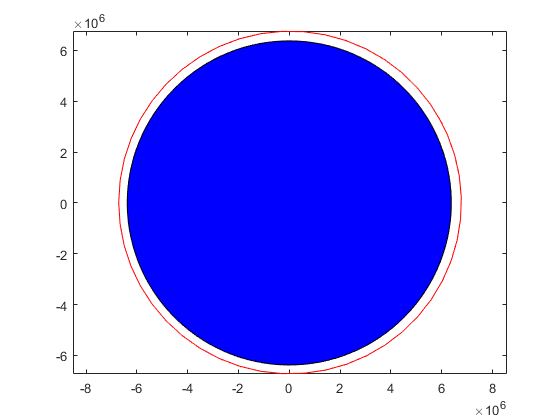
\includegraphics[width=1\linewidth]{./1_kreisbahn}
\caption{Eine Kreisbahn um die Erde}
\label{fig:1_Kreisbahn}
\end{figure}


\subsubsection{Versuch 2 - Entfliehung der Erde}
In diesem Versuch soll der Parameter $v_0$ bestimmt werden, sodass der Satellit gerade der Erde entflieht. Dafür werden folgende Startparameter 
 $\delta = 30^\circ, h_0 = 400km \Theta = 0^\circ $ und eine Simulationszeit $1 \cdot 10^6$ von angenommen werden.
 
 Das gewünschte Verhalten zeigt sich bei einer Startgeschwindigkeit $v_0$ von  $10,85 \dfrac{km}{s}$ und einer Simulationszeit von $1 \cdot 10^6$ wie in Abb. \ref{fig:1_Entfliehung}.
 
\begin{figure}[H]
\centering
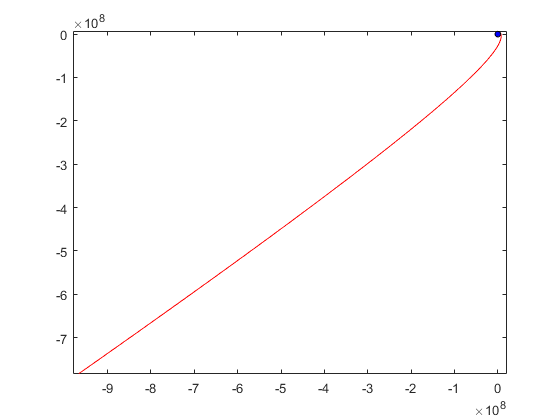
\includegraphics[width=1\linewidth]{./1_entfliehung}
\caption{Der Satellit entflieht gerade der Erde}
\label{fig:1_Entfliehung}
\end{figure} 


\subsubsection{Versuch 3 - Erdumrundung innerhalb eines Tages}
In diesem Versuch sollen die Parameter $h_0$ und $v_0$ so gewählt werden, dass der Satellit genau einen Tag benötigt um die Erde zu umkreisen.

Es ergab sich, dass der Versuch mit den folgenden Parametern durchgeführt werden muss um das gewünschte Ergebnis zu erreichen.
 $\delta = 30\circ, h_0 =  \Theta = 0^\circ $ 
 
 Um die Erde in genau einem Tag zu umrunden haben wir die Parameter $h_0 = 38.000 km$ und $v_0 = 2,85 \dfrac{km}{s}$ genutzt. Das Ergebnis ist in Abb. \ref{fig:1_einTagKreisbahn} dargestellt.

\begin{figure}[H]
\centering
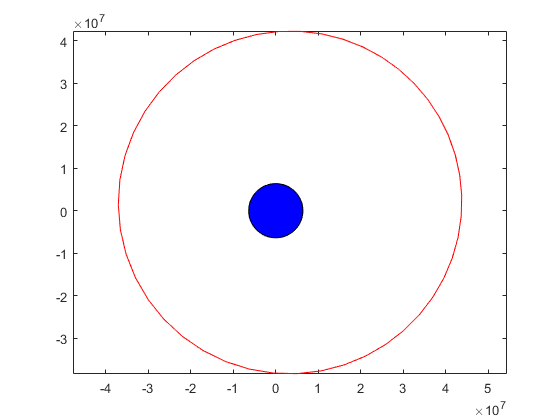
\includegraphics[width=1\linewidth]{./1_einTagKreisbahn}
\caption{Der Satellit umkreist innerhalb eines Tages die Erde}
\label{fig:1_einTagKreisbahn}
\end{figure}

\section{Teilaufgabe 2 - Mondumkreisung}
In der Teilaufgabe 2 ging es darum das Modell aus Aufgabe 1 so umzubauen, dass der Satellit nicht mehr nur um die Erde sondern nun auch um den Mond kreist. Dafür wurden folgende Parameter hinzugefügt:

Mondposition(fest)
\begin{align}
x_{M} = (0,-380000)^T km
\end{align}

Mondmasse
\begin{align}
m_{M} = 7,3480 \cdot 10^{22} kg
\end{align}

Dabei ist zu beachten, dass der Mond als feststehend angesehen wird.

\subsection{Veränderungen am Modell - Beschleunigung}
Um der Simulation eine Mondumkreisung hinzuzufügen muss die Funktion Beschleunigung modifiziert werden in dem der jetzigen Formel der Einfluss des Mondes hinzugefügt wird.

Die Beschleunigungs-Formel der Erde beschreibt sich als:

\begin{align}
a = G \cdot \dfrac{m_E \cdot m_S }{r^2_{SE}} \cdot \vec{e_{SE}}
\end{align}

Die Formel des Mondes wäre dann

\begin{align}
a = G \cdot \dfrac{m_M \cdot m_S }{r^2_{SM}} \cdot \vec{e_{SM}}
\end{align}

dabei ist $m_M$ die Masse des Mondes, $r_{SM}$ die Entfernung des Satelliten zum Mond und $ \vec{e_{SM}}$ der Einheitsvektor vom Satelliten zum Mond.
Aus der Formel zur Berechnung der Kraft

\begin{align}
\Sigma{F} = m \cdot a
\end{align}

Ergibt sich wie bereits vorher die Berechnung, nur das hier die Kräfte addiert werden die auf den Satelliten wirken.

\begin{align}
a = \Sigma{F}_{SE} + \Sigma{F}_{SM}
\end{align}

Somit wird, genau wie für die Erde auch für den Mond die Kraft berechnet die auf den Satelliten wirkt und addiert. Daraus ergibt sich die Beschleunigung.


\subsection{Durchführung}

Für die Darstellung der Simulation wird das bereitgestellte Matlab-Script $ErdMondBahn.m$ genutzt und die Simulation mit den Voreinstellungen 
 $\delta = 30^\circ, h_0 = 150km$
 
Mit einer Startgeschwindigkeit $v0 = 10,95$ und einem Flugwinkel von $\Theta = 26^\circ = $ fliegt der Satellit eine 8-förmige Schleife um den Mond und zurück zur Erde. Dabei dauert die Mondmission 9 Tage. Folgende Abbildung veranschaulicht das Ergebnis.

\begin{figure}[H]
\centering
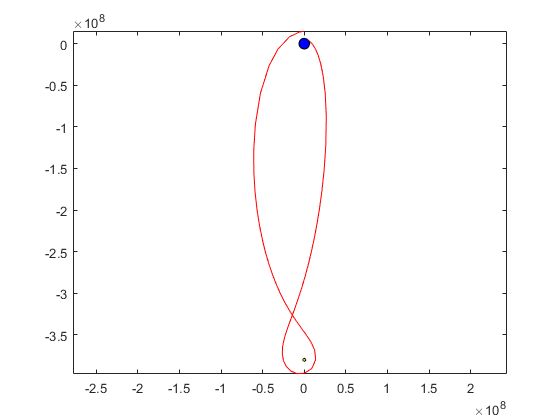
\includegraphics[width=1\linewidth]{./2_MondErdeAcht}
\caption{Der Satellit fliegt eine acht zum Mond und wieder zur Erde zurück}
\label{fig:2_MondErdeAcht}
\end{figure}

\section{Teilaufgabe 3 - Crazy Pendulum}
In dieser Teilaufgabe gilt es, die Bewegung einer Pendelkonstruktion zu berechnen. Der Versuchsaufbau ist in Abb. \ref{fig:3_Versuchsaufbau} zu sehen. In diesem Aufbau übt immer nur eine der Federn Zugkraft auf die Seiltrommel aus, während die andere Feder keine Kraft ausübt. Befindet sich das Pendel in senkrechter Position, dann übt keine der Federn eine Kraft aus. Der Einfluss der Pendelstange und der Seiltrommel werden nicht beachtet.

\begin{figure}[H]
\centering
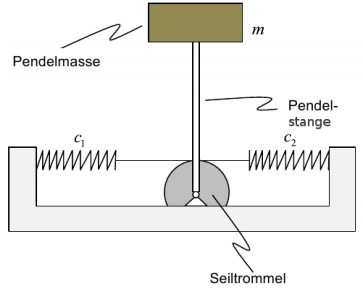
\includegraphics[width=0.5\linewidth]{./3_Versuchsaufbau}
\caption{}
\label{fig:3_Versuchsaufbau}
\end{figure}

\subsection{Gegebene Versuchskonfiguration}
Dieser Versuch wurde mit folgenden Parametern durchgeführt:
\begin{itemize}
\item $L = 1m$
\item $m = 10kg$
\item $r = 0.3m$
\item $w = 0.3m$
\item $h = 0.2m$
\item $c_{1} = 5000 N/m$
\item $c_{2} = 500\ 000N/m$
\item $\varphi(0) = 45^\circ$
\end{itemize}

\subsection{Freikörperbild}
%TODO: zeichnen und einfügen

\subsection{Formeln}
$c$ ist abhängig von $\varphi(t)$: es gilt entweder $c_{1}$ oder $c_{2}$.
\begin{align}
M_{p} = m \cdot g \cdot sin(\varphi) \cdot (L + \dfrac{h}{2})\\
M_{s} = -\varphi \cdot c \cdot r^2\\
M_{g} = M_{p} + M_{s}\\
J_{p} = \dfrac{1}{12} \cdot m \cdot (h^2 + w^2)\\
J_{g} = J_{p} + m \cdot (L + \dfrac{h}{2})^2\\
a = M_{g}/J_{g}
\end{align}
$a$ wird in der Einheit $Grad/s^2$ angegeben.

\subsection{Simulink-Modell}
Die Berechnung von $a$ erfolgt in der Embedded-MatLab-Function \textit{fcn}.

\begin{figure}[H]
\centering
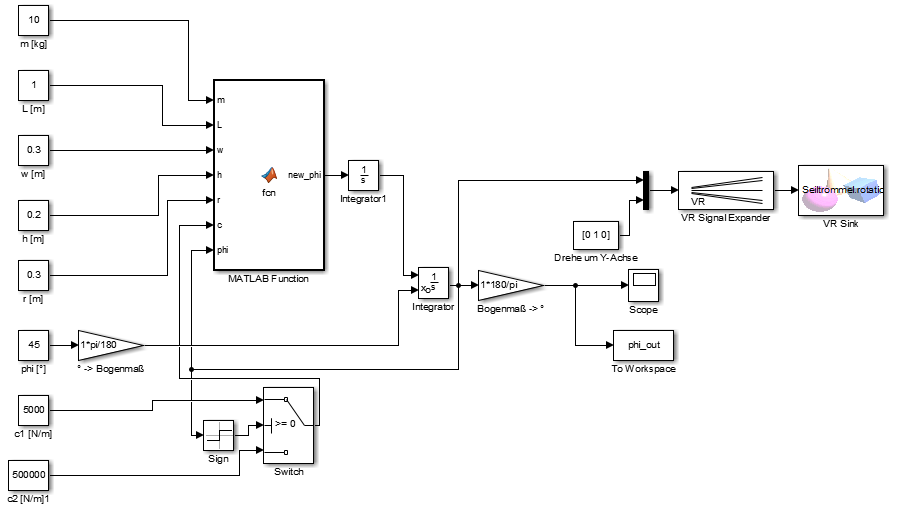
\includegraphics[width=1\linewidth]{./3_Modell}
\caption{}
\label{fig:3_Modell}
\end{figure}

\subsection{Plot des Ergebnis}
Die Abbildung \ref{fig:3_Plot} zeigt $\varphi(t)$ des Modells als Plot. Die Abstände und Maximalstellen der Kurve verändern sich während der Laufzeit nicht nennenswert. Sie bleiben nahezu gleich, eine Veränderung ist nur an der dritten Nachkommastelle zu sehen.

\begin{figure}[H]
\centering
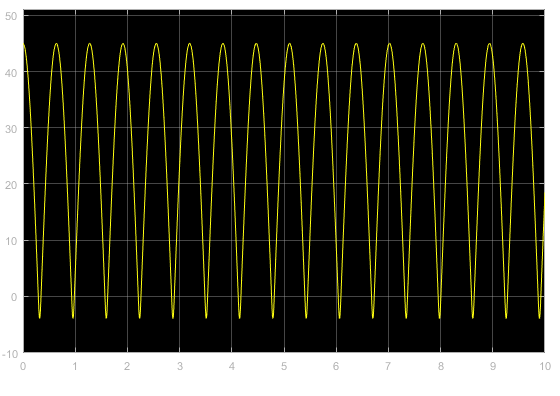
\includegraphics[width=0.5\linewidth]{./3_Plot}
\caption{}
\label{fig:3_Plot}
\end{figure}

\section{Teilaufgabe 4 - Schwingungsgedämpfter Tisch}
In dieser Teilaufgabe wird ein schwingungsgedämpfter Tisch simuliert. Der Versuchsaufbau ist in Abb. \ref{fig:4_Versuchsaufbau} zu sehen. Der Startbewegungsimpuls wird über \textit{u} gegeben. Die Massen $m_{1}$ und $m_{2}$ reagieren darauf mit den Auslenkungen $x_{1}$ und $x_{2}$.

\begin{figure}[H]
\centering
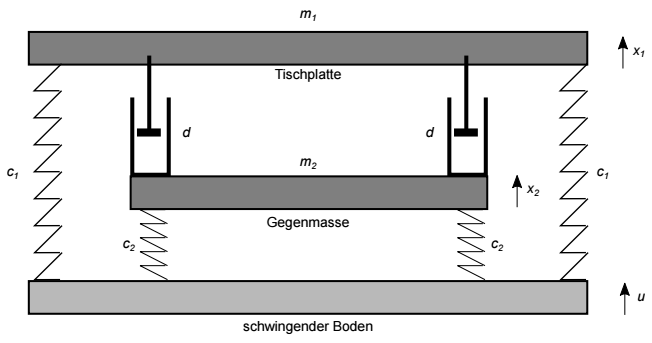
\includegraphics[width=0.5\linewidth]{./4_Versuchsaufbau}
\caption{}
\label{fig:4_Versuchsaufbau}
\end{figure}

\subsection{Gegebene Versuchskonfiguration}
Dieser Versuch wurde mit folgenden Parametern durchgeführt:
\begin{itemize}
\item $c_{1} = 15\ 000 N/m$
\item $c_{2} = 10\ 000 N/m$
\item $d = 600 Ns/m$
\item $m_{1} = 60 kg$
\item $m_{2} = 450 kg$
\end{itemize}

\subsection{Freikörperbild}
%TODO: zeichnen und rein damit

\subsection{Formeln}
Folgende Formeln werden zur Berechnung der einzelnen Komponenten verwendet:

\begin{align}
\Delta x_{1} = u - x_{1} \\
\Delta x_{2} = u - x_{2}\\
\Delta v = v_{1} - v_{2}\\
F_{G1} = m_{1} \cdot g\\
F_{G2} = m_{2} \cdot g\\
F_{c1} = 2 \cdot \Delta x_{1} \cdot c_{1}\\
F_{c2} = 2 \cdot \Delta x_{2} \cdot c_{2}\\
F_{D} = 2 \cdot \Delta v \cdot d
\end{align}

Ruhelage Tisch:
\begin{align}
x_{1}(0) = \dfrac{m_{1} \cdot g}{c_{1} \cdot 2}
\end{align}

Ruhelage Gegengewicht:
\begin{align}
x_{2}(0) = \dfrac{m_{2} \cdot g}{c_{2} \cdot 2}
\end{align}

Beschleunigung Tisch:
\begin{align}
a_{1} = \frac{-F_{G1} - F_{D} + F_{c1}}{m_{1}}
\end{align}

Beschleunigung Gegengewicht:
\begin{align}
a_{2} = \frac{-F_{G2} + F_{D} + F_{c2}}{m_{2}}
\end{align}

\subsection{Simulink-Modell}
Die Berechnung von $x_{1}(t)$ erfolgt in folgendem Simulink-Modell:

\begin{figure}[H]
\centering
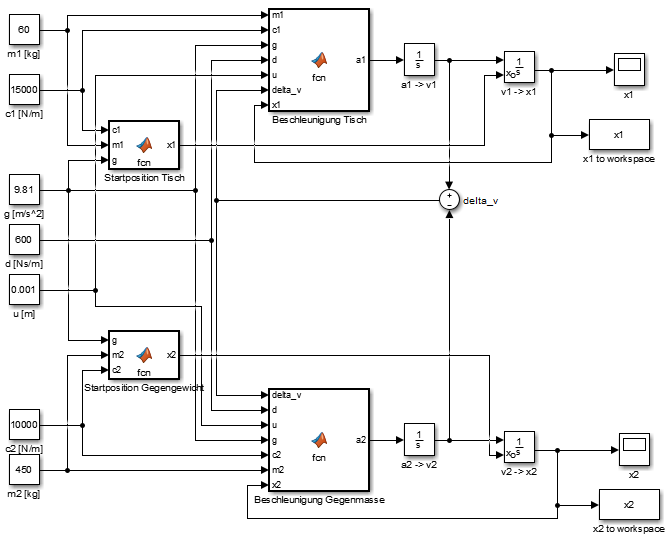
\includegraphics[width=1\linewidth]{./4_Modell}
\caption{}
\label{fig:4_Modell}
\end{figure}

\subsection{Plot des Ergebnis}
Die Abbildung \ref{fig:4_Plot} zeigt wie sich die Auslenkung von $x_{1}$ durch den Anstoß von $u$ verändert, bis der Tisch sich wieder in seiner Ruheposition befindet.

\begin{figure}[H]
\centering
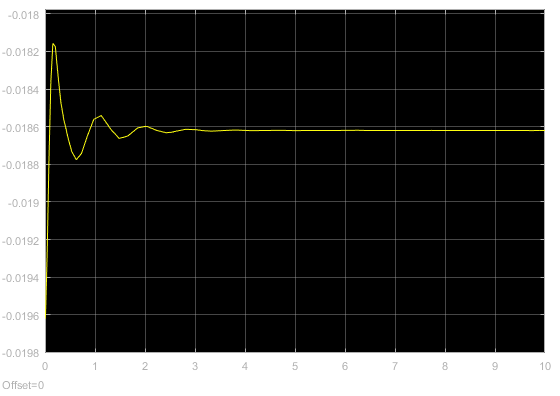
\includegraphics[width=0.5\linewidth]{./4_Plot}
\caption{}
\label{fig:4_Plot}
\end{figure}

\end{document}
